\documentclass{article}
\usepackage[final]{neurips_2023}
% \usepackage[margin=0.5in]{geometry} 
\usepackage{amsmath,amsthm,amssymb}
\usepackage{graphicx}
\usepackage{colortbl}
\usepackage{xcolor}
\usepackage{multirow}
\pagenumbering{gobble}

% Makes stuff clickable
% \usepackage{hyperref}
% \hypersetup{
%     colorlinks,
%     citecolor=black,
%     filecolor=black,
%     linkcolor=black,
%     urlcolor=black
% }

\title{FREEZE!: Pretrained Language Models as Frozen Feature Extractors for Semantic Tasks}
\author{
    Hayden McDonald\\hayden\_mcdonald@brown.edu \And
    Nicholas Marsano\\nicholas\_marsano@brown.edu\And
    Oliver McLaughlin\\oliver\_mclaughlin@brown.edu
}

\begin{document}

\maketitle

\begin{abstract}
    We investigate whether frozen language models can effectively serve as feature extractors for semantic tasks without any fine-tuning. By treating intermediate activations from different layers as independent sources of semantic information, we combine autoencoder pretraining with siamese networks to learn semantic representations. Using GPT2-medium as our base model, we achieve 76.86\% Pearson correlation on the Semantic Text Similarity Benchmark (STSB) using a model containing less than 7\% of GPT2-medium's parameter count. Our approach also produces an interpretable similarity measure for GPT2-medium's intermediate activations that aligns with human judgments of semantic similarity.
\end{abstract}
% \setcounter{secnumdepth}{4}
% \tableofcontents

\section{Introduction}
Our project is an investigation into a few related areas. In short, we wanted to see if we could develop an architecture that could take the intermediate activations of a pre-trained decoder-only large language model (Henceforth LLM) and use them to do text-embedding tasks. We chose semantic sentence similarity (STS) as our primary focus and motivation because of its simplicity. This task involves training a model to rate the semantic similarity of a pair of sentences. Importantly, in contrast to most other work using LLMs for text embedding, we are \textit{not} fine-tuning the model. We are simply taking a subset of the intermediate activations and treating them as a kind of \textit{"feature extracted"} (frozen) representation.

We chose this idea for several reasons.
\begin{enumerate}
    \item Our original motivational question was: \textit{"Do ‘similar’ prompts (to human readers) have ‘similar’ (under some metric) representations to a given language model?"}. By training a sentence-similarity model on LLM activations, we believed we could make progress on answering this question by \textit{learning} a transformation of the activations that correlates to semantic similarity.

    \item \textit{If} we could train a small model to interpret a given LLM's activations and produce a useful text embedding (or set of embeddings) from them, we could skip costly fine-tuning and simply pre-train and fine-tune the small "interpreter" model. Pretrained small LLMs are cheap to do forward passes on and very plentiful, so if we could \textit{just} use the intermediate activations and not have to do backward passes we could get a lot of functionality for very little compute.
    
    \item We also wanted to investigate the question: \textit{Do multiple intermediate activations perform better than just the last?} Typically when doing finetuning or transfer learning you remove the classifier end and use the last intermediate representation as your "feature extracted representation". We wanted to see if there was any performance benefit in using \textit{multiple layer's} worth of representation. This is clearly the case in the finetuning setting \cite{tang2024poolingattentioneffectivedesigns} but it's unclear if it will work here.
    
    \item From an interpretability standpoint, most distance or similarity measures (E.g cosine similarity) do not correlate strongly with \textit{human ideas} of similarity (Figure \ref{fig:raw-corr}). By training a similarity learner on LLM activations, grounded in human ideas of similarity, we hoped to produce a more interpretable measure of similarity for LLM activations.
    
    \item There just isn't that much work on this particular topic. For this task you'd typically finetune the LLM using LoRA \cite{hu2021loralowrankadaptationlarge} or simply just use an existing text embedding model. We hoped to discover interesting properties and learn a lot about what it's like to try and \textit{"disentangle"} an LLM's intermediate activations into something useful by pursuing this project. \footnote{There was only one paper we could find doing a similar setup -- extracting latents from an LLM and applying them to a task -- but it is very low quality and does not reveal many of the important details \cite{gpt2malware}. There are many papers \textit{like} this one (\cite{lu2021pretrainedtransformersuniversalcomputation} comes to mind) but almost none completely freeze the entire model and "start from scratch" as we did here.} We're not really interested in \textit{what} information is \text{where}, we just want to see \textit{if it's useable} for a simple task like STS.
    
\end{enumerate}
We chose \verb|gpt2-medium| (355M parameters) as our \textit{"base model"} for study because Oliver was familiar with its architecture and it readily fit onto all of our GPUs. We also did minor experiments on \verb|qwen2-0.5B| (391M parameters). Moreover we chose \verb|gpt2-medium| because of its very low quality text generation ability and verifiably low quality embeddings \cite{ethayarajh2019contextualcontextualizedwordrepresentations} (This paper tests the larger \verb|gpt2| base model which is more powerful. Our model is a smaller, less performant version of that). It was not at all a priori obvious to us that its representations would be fit for this task.


\subsection{Problem Setup} \label{Setup}
Figure \ref{fig:raw-corr} was our "starting point". This figure depicts the correlation between two important quantities for our investigation:
\begin{enumerate}
    \item The cosine similarity of two sentences' latent representations (See \ref{latent} for more information on this representation)
    \item A human rated similarity score for those same two sentences (See \ref{STS-section})
\end{enumerate}
For each layer we computed the mean correlation between these two quantities for more than five thousand sentence pairs. This is essentially the problem we are trying to solve -- \textit{How can we transform these latent representations into something useable for semantic text similarity?}

In short, we're trying to solve the problem of "low quality" embeddings in small LLMs like \verb|gpt2-medium| by finding an architecture which can leverage the information contained within its latents. Our target task for this experiment is semantic text similarity and we will measure success through our performance on the STSB \cite{STS} benchmark. To do this we trained a similarity learner on the STS dataset with some added unsupervised pretraining. We believe that if we can take these latent representations generated by \verb|gpt2-medium| and train a model to effectively use them that this would be evidence of these embeddings being much higher quality than originally expected in terms of their information content.

\section{Related Work}
% Related Work: Are you aware of any, or is there any prior work that you drew on to do your project?
%     Please read and briefly summarize (no more than one paragraph) at least one paper/article/blog relevant to your project.
Reusing pretrained LLMs for semantic tasks like STS is nothing new. There is extensive literature about finetuning and retraining
these models for a variety of new tasks \cite{reimers2019sentencebertsentenceembeddingsusing}, \cite{tang2024poolingattentioneffectivedesigns}. Moreover using decoder-only models for embedding tasks is common, with works like
SGPT \cite{muennighoff2022sgptgptsentenceembeddings}, LLM2VEC \cite{LLM2Vec}, LLMEmbed \cite{LLMEmbed} etc. exploring this idea as well as "meta-techniques" for improving these embeddings like Mitchell et. al's paper on how repeating a given piece of text within a prompt improves downstream benchmark performance after collecting a truncated subset of the generated latents \cite{RepImprovesLLM}. It is also well known that GPT-2 produces incredibly low quality embeddings \cite{ethayarajh2019contextualcontextualizedwordrepresentations} and even basic exploration shows that the smaller \verb|gpt2-medium| produces very low quality text generation.

Our work also takes inspiration from Adapters \cite{houlsby2019parameterefficienttransferlearningnlp} and other parameter-efficient fine-tuning methods. Adapters take the theoretical stance that large pretrained models have most of the information needed to accomplish tasks within their domain. However, they just need a little bit of direction and transformation in the intermediate activations to make their representations more amenable to the particular task. So, instead of fine-tuning a base model to accomplish a new task, one can instead insert "adapter modules" - small feed-forward neural networks situated between layers - and train those parameters instead. This keeps most of the information flow of the original model intact but modifies how information passes through the layers to optimize performance on the target task. 

\begin{figure}[!htb]
    \centering
    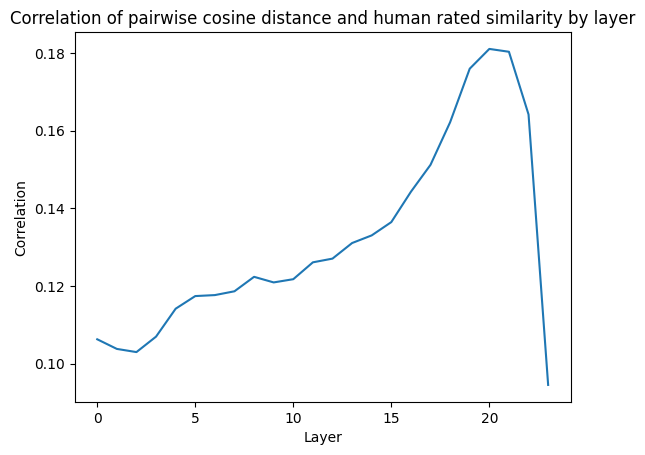
\includegraphics[width=0.65\linewidth]{raw_cosine_sim.png}
    \caption{\textbf{The problem we are ultimately trying to solve}. Layerwise average correlation between gpt1-medium's embeddings and their cosine similarity vs. human similarity score for the STS training pairs}
    \label{fig:raw-corr}
\end{figure}    


\section{Data}
We have three major datasets that we used for both pretraining and supervised STS training.
\begin{enumerate}
    \item STSB \cite{STS} -- A standard sentence similarity benchmark with associated training and test sets. The sentence data is scraped from articles and news headlines and was rated by humans for their semantic similarity.

    \item GenericsKB \cite{bhakthavatsalam2020genericskbknowledgebasegeneric} -- A 'generic sentence' dataset of which we used twenty-thousand examples. These sentences are varied in length and content and serve as our baseline distribution of sentence data.

    \item SNLI \cite{snli} -- An inference relation dataset. Used in a pretraining experiment and in Sentence-BERT \cite{reimers2019sentencebertsentenceembeddingsusing}.Most relevant to our discussion is that this dataset was used as a pretraining task in the Sentence-BERT paper \cite{reimers2019sentencebertsentenceembeddingsusing}.
\end{enumerate}

\subsection{Semantic Text Similarity Benchmark (STSB)} \label{STS-section}
The main task we targeted was STSB \cite{STS}, which is a benchmark for semantic text similarity. It's comprised of pairs of sentences and a human-rated "similarity score". For example:
$$
(\text{s1='A plane is taking off.'}, \text{s2='An air plane is taking off.'}, \text{sim}=1.0)
$$
The performance metrics for STS are typically Spearman's rank correlation coefficient and normal Pearson correlation between the predicted similarities of pairs of sentences and the human rated similarities. State of the art for this task is around \verb|90 - 92%| in both spearman and pearson according to the MTEB leaderboard \cite{muennighoff2022mteb}.

\subsection{Data Collection and Pipeline} \label{latent}
Our data pipeline is fairly simple. We're treating \verb|gpt2-medium| as a feature extractor, so for each piece of text for any task, we simply pass that text through the model and extract a latent representation from the intermediate activations at each layer. We chose to take the \textit{last token at each layer, after the residual connection} (Henceforth called a \textit{latent}). This strategy is not original and is fairly standard in the \textit{fine tuning} literature \cite{LLMEmbed}. We expected it to do fine for our task given that \verb|gpt2-medium| uses causal attention (and thus the last token has "seen" all of the previous tokens), even though we're not fine tuning. This gives us, for each sentence, twenty-four \verb|1024| dimensional vectors (\verb|n_layers x d_model|, \verb|gpt2-medium| has twenty-four layers). One of the main challenges we wanted to overcome by taking this project on was finding a sensible way to \textit{actually use} such a high volume and dimensionality of data.

We found no benefit from normalizing our activation data (I.e. center and then scale to unit variance) so we decided to not do so in our final model training. Rerunning our analysis confirms that external data normalization does not increase performance in our task (Likely due to the layer normalization employed by our autoencoders).
% Data: What data are you using (if any)?

%     If you’re using a standard dataset (e.g. MNIST), you can just mention that briefly. Otherwise, say something more about where your data come from (especially if there’s anything interesting about how you will gather it).
%     How big is it? What kind of preprocessing was required?

\section{Methodology}
% Methodology: What is the architecture of your model?
%     How are you training the model?
%     Justify your design. Also note some things you tried that may or may not have worked.
The key insight behind our approach is that different layers in transformer models encode distinct types of information, with each layer potentially discarding or transforming information from previous layers as it builds towards its final objective. This idea is most clearly shown in Anthropic's work on Sparse Autoencoders for interpretability of LLMs \cite{bricken2023monosemanticity} wherein different layers are shown to possibly be responsible for representing different and specific information.

Rather than assuming later layers contain all necessary information, we hypothesized that earlier layers might preserve valuable semantic features that get filtered out during the progression through the model. While this is similar in concept to adapter models \cite{houlsby2019parameterefficienttransferlearningnlp}, our approach has a key advantage: since we're not constrained by the need to maintain the original model's information flow, we can treat each layer's representational space as fully independent. This allows us to potentially capture and utilize semantic features that might otherwise be lost or transformed as information propagates through the model's layers. Moreover, our space of possible models is much larger than a traditional adapter setup because we are not constrained by any uninvertable or irrelevant transformations made in between layers.

\subsection{Training and Loss function} \label{Loss} \label{Training}

\subsubsection{Training}
Our general training scheme was the following:
\begin{enumerate}
    \item Pass whatever example sentence for the current task through \verb|gpt2-medium|
    \item Extract the latents (Described in Section \ref{latent}) from each layer. We take these latents and completely decouple them from the base model. They are effectively just a set of vector representations of the input. No gradient is passed back through \verb|gpt2-medium|. In our actual experiments we pre-computed all of these latents and saved them to disk.
    \item Pass those latents into our model.
\end{enumerate}
To train our model to do STS we pass in both pairs of sentences to \verb|gpt2-medium| as described above, pass those latent vectors into our model and extract a scalar similarity value. We then do supervised training where the ground truth is the human-rated similarity value of the two sentences as given by the STSB dataset.

\subsubsection{Loss function}
Our loss function evolved throughout our experiments. Initially, we used mean squared-error (MSE) loss between the predicted similarities for a sentence pair and the human-rated similarities from the STSB dataset. For our final model, however, our loss function for supervised STS training departs from traditional MSE in that we only minimize the \text{variance of the residuals}, instead of both variance \text{and} bias which are traditionally minimized when using MSE. While our model's performance is evaluated using both Pearson and Spearman correlation (which measure linear and monotonic relationships respectively), we found that simply minimizing residual variance without enforcing zero bias led to strong performance on both metrics. 

Empirically we found that our residuals centered themselves near zero even though we didn't enforce this directly. We also found that taking the log of this value improved training stability and overall performance. We attribute this to the fact that the variance here is bounded between zero and one\footnote{Our residuals are bounded within $[-1, 1]$, so the highest variance distribution here would be $P(-1) = P(1) = 0.5$ which has a variance of one}, so taking the logarithm here makes the signal to move towards zero significantly stronger. Our final loss function is then:
$$
\mathcal{L}(\theta) = \log(\text{Var}(y_\theta - y))
$$
Where $y_\theta$ is the predicted similarity scores and $y$ is the ground truth. We only saw meaningful improvement with this new loss metric on the final architecture, so our experimental results reported for all but the last model used MSE.

\subsection{Architecture} \label{Architecture}
Our architecture was decided through a series of experiments and trial and error. We tried to only make architectural decisions which were, in some way, \textit{principled} -- I.e. we had a decent reason for making that particular change.

\subsubsection{First iteration}
Our first architecture was incredibly simple -- Just take the layerwise cosine similarities described in Section \ref {Setup} and pass them through an MLP to do basic weighting and statistical correlation. We felt this was reasonable because although the individual correlations were quite weak, it wasn't clear to us that each layer was correlating \textit{to the same content}. In the same way that many weak models can be combined to create a strong one, we figured that a simple MLP would be able to decipher some of the more complicated relationships, even just through the layerwise similarities. This model was quite simple, just a two layer MLP (We did not find better performance with deeper models) that took the twenty-four layerwise cosine similarities from \verb|gpt2-medium|'s respective latents and outputted a sigmoided single scalar. This was trained using the scheme described in Section \ref{Training}. This model significantly improved upon baseline, giving us a test set pearson correlation of \verb|39.2%| and spearman of \verb|42.06%| ($p<< 0.001$)

\subsubsection{Layerwise Siamese Networks}
After the previous architectural experiment, we figured that we were probably bottlenecked by the representation of our base model, necessitating a transformation. Inspired by prior work on Siamese networks for semantic tasks \cite{reimers2019sentencebertsentenceembeddingsusing}, we decided to modify our architecture by applying siamese networks to each layer, computing the cosine similarities of \text{those} representations, and then finally passing those cosine similarities into a weighting/pattern matching MLP as described above. The intuition here is that each layer probably contains meaningfully different and useful information, as evidence by weighted cosine doing better than any particular layer. So, if we learn a nonlinear transformation of each layer's particular space through supervised STS training, we might be able to extract a better representation for this task and have overall better downstream performance.

This architecture achieved a \text{significant} performance increase, moving our pearson and spearman on the test set to \verb|71.63%| and \verb|69.72| ($p << 0.001$) respectively.

\subsubsection{Autoencoder pretraining and the final model}
\begin{figure}
    \centering
    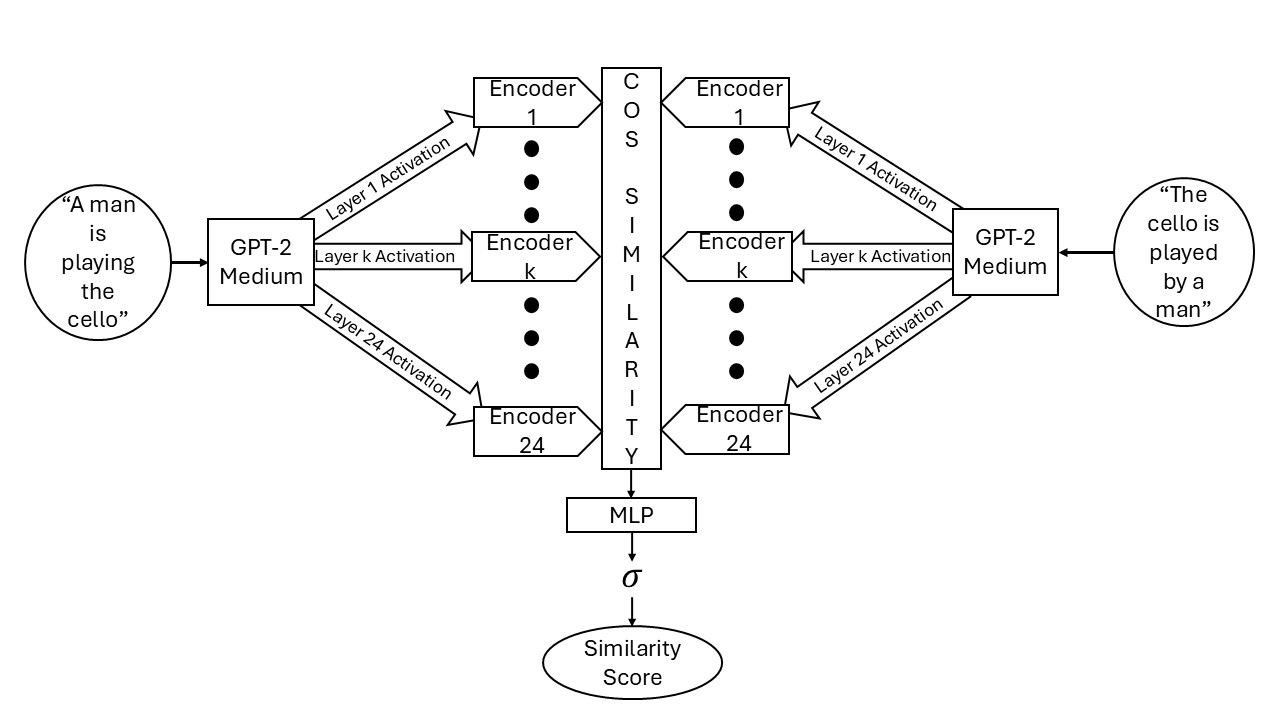
\includegraphics[width=1\linewidth]{model-diagram.jpg}
    \caption{Final Model Diagram}
    \label{fig:model-diagram}
\end{figure}

We then realized that although this architecture was training quite well, it was likely the case that inputs which were significantly different from those in the input distribution would likely not be well represented by our siamese networks. This then inspired us to change our training strategy. Our current strategy \text{coupled} our representation learning and our supervised STS learning. That is, the model had to both learn a good representation of the input whilst also learning how to orient examples spatially to reflect semantic similarity. We then decided to break this up by first training a set of layerwise autoencoders over twenty-thousand "generic" sentences from the GenericsKB \cite{bhakthavatsalam2020genericskbknowledgebasegeneric} dataset. These sentences were similar in length and complexity to the STS training set that we felt it was an appropriate 'pretraining' dataset. We trained the autoencoders to reconstruct each layer's latent for each sentence (I.e. twenty-four autoencoders, each trying to reconstruct their respective layer's latent). We then did this pretraining and took the encoder part of each autoencoder and treated it as our new siamese network. Each autoencoder had a bottleneck of $256$ hidden units.

Immediately, our results were \textit{indistinguishable} from the results of the previous section. We then produced Figure \ref{fig:autoencoder-loss} and realized that the layerwise losses for each autoencoder increased exponentially as the layers went on. This inspired us to, among many other things that did not work, widen the bottleneck of the last twelve autoencoders from $256$ to $512$. This then finally showed a performance increase to \verb|75.36%| pearson and \verb|73.21%| spearman. Our final change was to incorporate the loss function switch described in Section \ref{Loss}, which brought us to a final pearson and spearman correlation of:
\begin{align*}
    &\text{Pearson} = 76.86\%\\
    &\text{Spearman} = 75.03\%\;,\; p << 0.001
\end{align*}
Moreover, this architecture actually ended up with more than $600,000$ fewer parameters when compared to our previous best model. Importantly, the \textit{only} way we saw an increase in downstream performance, after many hyperparameter experiments and automated tuning, was to \textit{widen the bottleneck at the later layers}. This heavily suggests that the information present at later latent vectors is not only much richer (And thus requiring many more bases to represent) but also incredibly important for semantic tasks. Critically, \textit{deepening} the autoencoders \textit{did not improve downstream performance}, even though doing so added millions of parameters. Only widening the bottleneck improved performance. Our model is depicted in Figure \ref{fig:model-diagram}.

\begin{figure}
    \centering
    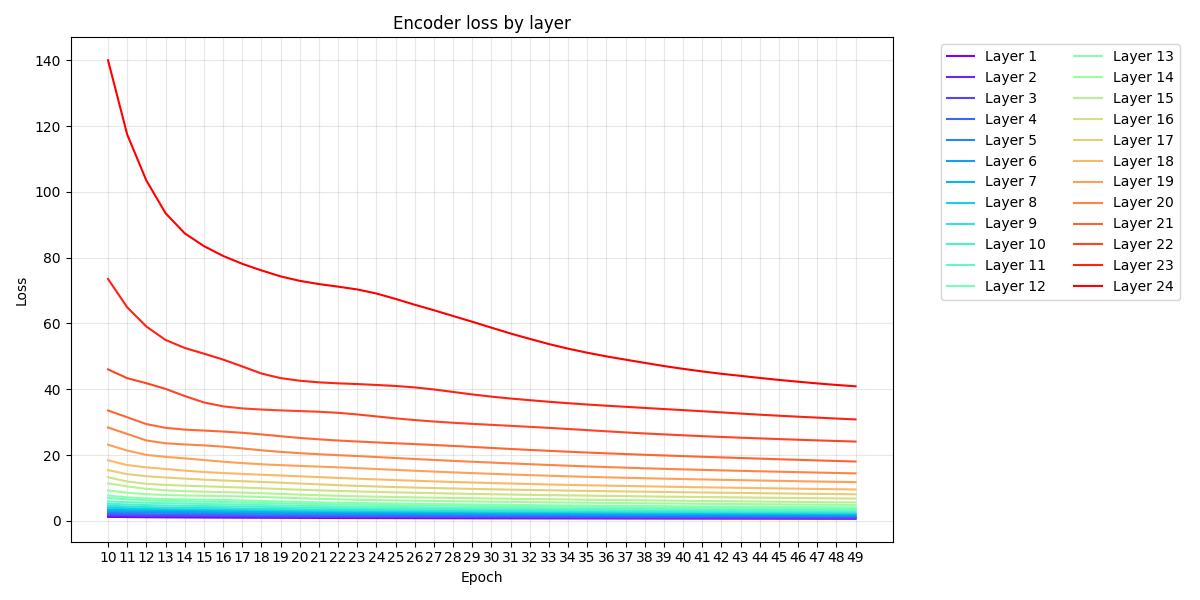
\includegraphics[width=1\linewidth]{encoder_loss.png}
    \caption{Autoencoder loss by layer. $\text{d}_\text{bottleneck} = 256$}
    \label{fig:autoencoder-loss}
\end{figure}

\subsection{Experiments that failed}

\paragraph*{Alternate Latent Choice}
We tried several choices of latent including mean and sum pooled accross all of the tokens at each layer. We found significantly worse performance from either approach. Intuitively this makes sense, only the last token has a "full picture" of the input and polluting that token with others would surely decrease performance. 

\paragraph*{Hyperparameter Optimization}
We ran several hyperparameter optimization/search runs on the autoencoders changing everything from their depth, dropout rate, width, etc. and found absolutely no benefit in downstream performance (Despite significant effort). We tried both manual approaches and automated approaches using Optuna. Interestingly, we \textit{did} see improvements in our autoencoder loss but did not see any downstream benefit -- Suggesting our informational bottleneck is either the incoming latents or the architecture itself.

\paragraph*{SNLI Pretraining}
Sentence-BERT \cite{reimers2019sentencebertsentenceembeddingsusing} pretrained its siamese networks on the SNLI \cite{snli} relation task to great benefit. We tried this with our layerwise approach and found success in the SNLI task but no downstream benefits for STS.

\paragraph*{Pooling and attention mechanisms}
We tried several schemes for pooling or otherwise combining both the latent representations coming from \verb|gpt2-medium| and our learned representations. One pooling strategy we tried (Inspired by the 'semantic subspaces' idea of Bolukbasi et. al \cite{bolukbasi2016mancomputerprogrammerwoman}) in the hopes of creating a single unified embedding was modifying the autoencoder training to instead of having twenty-four individual vectors to decode, we simply up-projected each encoder's bottlenecked output and summed accross each layer. This gave us a single high dimensional vector which we then fed into each "decoder", which was was trained to reconstruct the original layer's embedding from the unified one. The idea was that the unified representation would be encouraged to reuse subspaces to carry each layer's individual information so that it could be appropriately decoded. This model performed worse than our best model with a Pearson correlation of roughly \verb|60%|. We do believe, though, that this scheme is probably the way forward if we want to expand to other tasks.

We also experimented with some of the attention and attention pooling strategies outlined in Tang et. al \cite{tang2024poolingattentioneffectivedesigns}. This did not do well when pooling either the original latents, nor the learned autoencoded representations.

\paragraph*{Fake Data}
At one point we were wondering if we just simply didn't have enough examples of semantically similar sentences to break our best score, so we tried a few data generation strategies to see if we could mitigate this problem. Most notably we tried adding a little bit of noise to the activations to see if the model would generalize better -- It didn't. We also tried modifying the prompts to change words or capitalization (To see if the difference in tokenization would change anything) -- It didn't.

\section{Results}
\subsection{Requirements for success}
Our main notion of success was performance on the STSB \cite{STS} benchmark as described in Section \ref{STS-section}. Pearson/spearman correlation are both reasonable measures of success on this task because they measure how consistent your model is with human-rated similarity notions, regardless of scale or center. State of the art on this task is \verb|90-92%| for both Spearman and Pearson correlation as of the writing of this document \cite{muennighoff2022mteb}. Our goal was to achieve at least \verb|60%| pearson correlation. We really did not have strong reasoning for why this might be a reasonable goal but preliminary results showed that at least \verb|40%| was possible so we decided that \verb|60%| was a reasonable stretch goal.

\subsection{Final Results}
We achieved a Pearson correlation on STSB's test set of \verb|76.86%| \footnote{We were able to score up to $77.1\%$ but were unable to consistently reproduce it. The score we report here is the one in our notebook.} and a Spearman correlation of \verb|75.3%| with a p-value of significantly less than \verb|0.0001|. Ablation studies confirm both the utility of the unsupervised pretraining and the benefit of using multiple layers\footnote{Doing meaningful ablation studies on our setup is difficult because our model is designed to train using multiple latents at a time. We tried just training a normal single-latent model and in every case performance suffered. That being said, to fully decide whether 'multiple layers are better than just one' would require investing significant time into tuning our setup to use a single latent. At least in this setup, we consistently found performance decreases when ablating any of the latents. Section \ref{answering-questions} offers more insight into this question.}, in either case removing that step (or any layer) decreases performance. Our results are summarized in Figure \ref{fig:final-reslts}. Our model's errors on the test set are quite favorably distributed, Figure \ref{fig:residuals} shows that the vast majority are centered near zero ($\mu = .06$, $\sigma = 0.197$) and the Q-Q plot shows that our model is distributed relatively symmetrically with thin tails, indicating no major over or underprediction. Contrary to our intuition, changing our loss function back to MSE did not bring the center of our residuals to closer to zero but instead just increased the variance.

We also performed some qualitative analysis on the highest error predictions (See Section \ref{error analysis} for more details) and note that although or model performs moderately well on the benchmark, it has clear and unavoidable limitations. Most notably, it has trouble distinguishing semantic and syntactic similarity and it did not learn to recognize identical sentences. Despite these limitations, we still consider our results a success because of our performance on STSB. Even though \textit{some} of our model's predictions are quite bad, the vast majority of them are quite good, hence our STSB performance.


\begin{figure}[!htb]
    \centering
    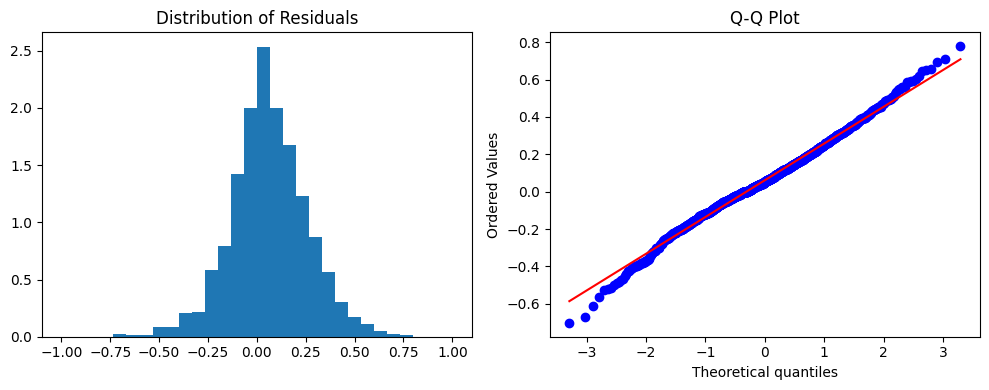
\includegraphics[width=.90\linewidth]{residuals.png}
    \caption{Density histogram and Q-Q plot of final model errors}
    \label{fig:residuals}
\end{figure}    


\subsection{Answering Our Original Questions} 
\subsubsection{\textit{Do 'similar' prompts have \ 'similar' representations?}}
Our results suggest that, yes, under a particular transformation (our model), \verb|gpt2-medium|'s latents do in fact correlate strongly with human notions of similarity. This implies that all of the necessary information to produce a decent sentence similarity model is encoded within the latent representations of the base model.

\subsubsection{\textit{Do multiple layers perform better than just the last one?}} \label{answering-questions}
This question was particularly interesting to us becuase if multiple layers did in fact perform better than just the final one, it would say quite a lot about the importance of information being lost during a forward pass.

In short, we found that using all layers works better than just picking one. Single-layer versions of our model (keeping the same architecture but only using one layer) performed notably worse, reaching only \verb|71%| correlation. At first, this seemed like a meaningful comparison, but we later realized it's not particularly informative - our full model has 24 times more parameters than the single-layer version, and more importantly, if some layers weren't useful, the model could simply \textit{learn to ignore them}. We now view the choice of which layers to include as just another hyperparameter to tune, rather than a fundamental architectural decision.

Interestingly, Figure \ref{fig:raw-corr} shows that the last latent in the residual stream was essentially \textit{useless} for this task. This may suggest that previous evaluations of GPT-2 for embedding tasks, among others, may be fundamentally limited by their choice of latent.

\begin{figure}
    \centering
    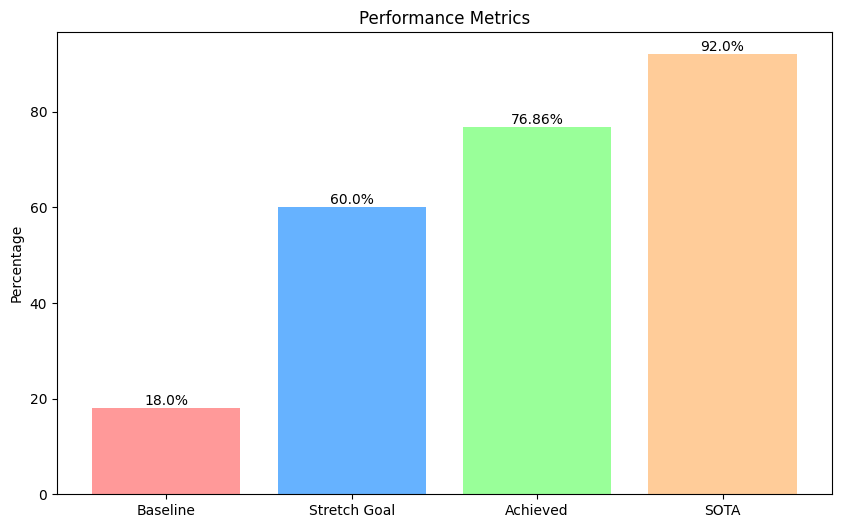
\includegraphics[width=.85\linewidth]{final_results.png}
    \caption{Final results -- Pearson correlation}
    \label{fig:final-reslts}
\end{figure}

\section{Ethics}
% Ethics: Choose 2 of the following bullet points to discuss; not all questions will be relevant to all projects so try to pick questions where there’s interesting engagement with your project. (Remember that there’s not necessarily an ethical/unethical binary; rather, we want to encourage you to think critically about your problem setup.)
%     What broader societal issues are relevant to your chosen problem space?
%     Why is Deep Learning a good approach to this problem?
%     What is your dataset? Are there any concerns about how it was collected, or labeled? Is it representative? What kind of underlying historical or societal biases might it contain?
%     Who are the major “stakeholders” in this problem, and what are the consequences of mistakes made by your algorithm?
%     How are you planning to quantify or measure error or success? What implications does your quantification have?
%     Add your own: if there is an issue about your algorithm you would like to discuss or explain further, feel free to do so.
There are two main societal impacts of this project. First, it addresses the relatively high barrier of entry for STS tasks by showing promise in lightweight methods that bypass the need for resource-intensive fine-tuning. This bypass offers a glimpse into the democratization of advanced NLP capabilities for researchers or organizations with limited computational resources. As more LLMs become open source, the barrier of entry to leverage them in practical applications can be lowered and allow for more innovation in smaller-scale environments. Second, the project addresses the advancement of model interpretability to increase trust in deployed models. By training an architecture to derive meaningful embeddings from intermediate activations, it contributes to the broader understanding of how LLMs encode semantic information. By helping to bridge the gap between machine representation and human comprehension, this project helps to further AI transparency as it plays a more dominant role in everyday life. 

\section{Discussion}

\subsection{\textit{"What did the model learn?"}}
An interesting question to ask here is \textit{What kind of semantic similarity did our model learn?} Although STSB has a particular idea of semantic similarity (Namely, that two sentences 'mean' the same thing), true \textit{"semantic similarity"} is not limited to just identical ideas being expressed in different ways. We could easily define semantic similarity to be in regards to the abstract character of the sentences, or of the \textit{ideas} they are conveying. For example, STSB labels the \textit{"semantic similarity"} of the following sentences as \verb|20%|:
\begin{verbatim}
    'Hawaii passes gay marriage bill', 'US Senate passes gay workers bill',
\end{verbatim}
Our model labels them at \verb|75.98%|. Which is \textit{"more"} correct? Although the literal content of the two sentences is different, they are quite similar in what they are conveying -- Bills being passed regarding LGBT civil rights. There are numerous examples exactly like this one. One weaker example is:
\begin{verbatim}
    'You will want to clean the area first.',
    'You will also want to remove the seeds.',
\end{verbatim}
Which STSB has rated at a similarity of \verb|0%|. Our model is less conservative in its estimate at \verb|56.01%|. Neither interpretation is wrong and clearly our model makes obvious and unavoidable errors (See Section \ref{error analysis} for more details) but in many contexts -- such as following steps in a recipe -- these sentences could be functionally identical, both indicating preparatory steps in a sequence.

This raises deeper questions about the nature of semantic similarity itself. Two humans, given different contexts or purposes (e.g., legal analysis vs. historical study), might rate these sentences quite differently. Our model's architecture, processing information across multiple transformer layers, may naturally capture these various levels of similarity -- from surface-level linguistics to broader themes. Of course this does not distract from the fact that our model is nowhere near state of the art, but it is a worthwhile question to ask either way. Clearly our training produced \textit{a particular interpretation of semantic similarity}, but which was it? Excluding clear errors, of course. We offer more insight into this in Section \ref{error analysis}.

\subsection{\textit{"What did we actually create?"}} \label{pathways}
Although our original motivation was in the vein of interpretability, our approach combines several potentially useful components:
\begin{itemize}
    \item A layerwise-independent\footnote{As opposed to Adapters, which are layerwise \textit{dependent}.} parameter-efficient approach to adapting existing LLMs to sentence similarity without fine-tuning
    \item A similarity measure for \verb|gpt2-medium|'s activations that aligns with human judgments of semantic similarity, potentially offering more interpretable insights into the model's representations
    \item A representation learning scheme for LLM activations that preserves the base model's weights and information flow while enabling task-specific adaptation
\end{itemize}
While our performance does not match state-of-the-art models, these techniques might prove useful for understanding and utilizing frozen LLM representations in other contexts. Our technique is also quite parameter efficient, using less than seven percent of the base-model's total parameter count. In future work we aim to see how far these individual components can be improved. 

\subsection{\textit{"What about a bigger base model?"} and the Representational Ceiling}
We ran many, many hyperparameter experiments on the autoencoders and did not find any benefit (despite significant effort) in downstream performance beyond the aforementioned widening of the bottleneck at later layers. This suggests an important limitation of our setup -- \textit{The representational capability of our base model}. In the finetuning scenario the entire "representational machinery" of the base model is appropriated for the new task. Millions of parameters are modified and retuned to throw away useless information (wrt the task at hand) and prioritize information that improves performance on the new selected metric. In our situation, we are \textit{"stuck with"} whatever representation the original training for \verb|gpt2-medium| produced. Critically, this representation is not tuned for semantic similarity tasks, but for next token prediction. It is likely that these two objectives require substantially different representations (and thus contextual information) of the input to perform well at.

A natural extension to our work would be to try a larger and more capable base model. Our initial experiments used \verb|qwen2-0.5B|, which performed significantly better than \verb|gpt2-medium| on both Pearson and Spearman correlation (\verb|+~2%| on both). However, this gap disappeared once we made the changes to the loss function described in Section \ref{Loss}. After rerunning the experiments with both base models and the new loss function, we found no meaningful difference between the two despite \verb|qwen2-0.5B|'s additional parameters. This likely suggests a limitation in our experimental setup for qwen2, given that we simply substituted the base model in our original architecture and only adjusted the input dimension of the autoencoders to match. A more thorough investigation of larger models would require architectural changes tailored to their specific parameter counts. We just wanted to assure that our approach was not uniquely suitable for \verb|gpt2-medium|.

% \subsection{\textit{"Why did increasing the bottleneck work"}}
% Couple of weird things here

% Loss COULD be explained by exponentially larger norms as layers go on

% COULD ALSO be explained by harder compression problem

% Maybe both??

% Increasing the bottleneck was the only way to improve performance, deeper didn't matter, suggesting the bottleneck was meaningful

\section{Reflection}
We're very happy with how this project turned out. There were a couple of scares here and there (one horrible incident of accidentally swapping our train and test sets for a few days comes to mind) but overall the performance we reached was significantly past our goal and we learned an incredible amount. We're quite proud of how we were able to take such a weak model and turn it around into a, though not state of the art, mostly capable STS model.

At the start of this project we made a pact to try and be principled with each decision that came our way. For example, we made it a rule to never just make a model deeper or wider for no reason. We tried to stay as minimal as possible throughout the whole project and we feel that paid off. We believe that every decision in our architectural design process (Mostly described in Section \ref{Architecture}) had good and clear motivation. We're also incredibly proud of our experimentation and overall scientific process.

If we had more time we would definitely choose to try and make our model a more general embedding model (Likely though some kind of pooling mechanism) and work towards applying it to the Massive Text Embedding Benchmark \cite{muennighoff2022mteb}. We have some other experiments that we briefly described in the section on architecture that we believe are the way forward in terms of overall performance, we just think they would take significant time and research effort to prove fruitful. Finally, we would do more thorough model comparisons (I.e. full-scale finetuning \verb|gpt2-medium| to the task, using our architecture with different base models) so we have a clearer picture of how our architecture stacks up against other choices. There aren't many models on the MTEB or STSB leaderboards that are similar to ours, so it's hard to get perspective. Even parameter count isn't necessarily a good measure of how close we are because the vast majority of our "parameters" are not trained.

We were quite surprised none of the pooling and attention mechanisms worked significantly better than our architecture. Our key takeaway from those experiments is that the finetuning literature relies on being able to shape the entirety of the representation present in the base model. When you can't control every part of the representation (as in our scenario where we're only "reading" the activations) attention and other linear-combination based methods (Such as sum or mean pooling) just don't make sense. The base model likely learns to use different tokens in the residual stream quite differently, likely not in a way that can just be arbitrarily combined.

Our biggest takeway by far from doing this project is that research is an incredibly fun and collaborative process. We all thoroughly enjoyed all the exploration, reading, experimentation, and rebuilding our mental models over and over to try and make good decisions. As for what we learned, we all believe we made significant progress in our understanding and ability in, among other things, training and debugging neural networks, transformer models, metric and similarity learning, reading and consuming research papers, scientific writing, and collaborative research.

\section{Division of Labor}
% Division of labor: Briefly outline who will be responsible for which part(s) of the project.
\begin{itemize}
    \item \textit{Oliver.}  Lead the research effort and designed and implemented the major architectural experiments. Took on most of the report writing.
    \item \textit{Hayden.} Lead the analysis effort and discovered the bottleneck in the autoencoders. Performed the first manual hyperparameter experiments and investigated intermediate correlations that helped improve our understanding of the model.
    \item \textit{Nick.}  Lead the automated hyperparameter optimization effort and proposed alternate approaches for improving our score. Performed a significant portion of the literature review and collected techniques and paths we could take.
\end{itemize}
Our group is quite happy with how the work was distributed and feel our individual strengths were able to be leveraged whilst also allowing each individual to specalize deeply into what they were interested in.

\newpage
\section{Appendix: Qualitative Analysis of Model Errors} \label{error analysis}
To better understand our model's limitations, we sorted all sentence pairs in the STSB test set by the absolute difference between predicted and true similarity scores. Below are the five pairs with the largest errors, representing our model's most significant failures.

\begin{verbatim}
"Not 'hiding the ball' on Russia: Obama",
"Obama says he's not 'hiding the ball' on Russia",
True similarity: 0.8800
Predicted: 0.2084

"Taiwan's economy grows 2.27% in April-June quarter",
"China's economic growth rebounds to 7.8% in latest quarter",
True similarity 0.2000
0.8955

'A man is laughing with a woman',
'A man and a woman laughing.',
True similarity: 0.9600
Predicted: 0.2572

'Supreme Court to Hear Voting Rights Act Case',
'Supreme Court to hear corporate human rights case',
True similarity: 0.2800
Predicted: 0.9893

"Hassan Rouhani wins Iran's presidential election",
'Maduro wins Venezuelan presidential vote',
True similarity: 0.0400
Predicted: 0.8193
\end{verbatim}
These are just the worst performing sentence pairs but they show a trend seen by browsing the top fifty or so. Clearly our model has a different idea of similarity than STSB does, but that model isn't always completely off base. Consider the last sentence pair in this set. Both sentences describe a particular figure winning a particular election. Obviously, semantically, these two sentences are nothing alike, they are describing two completely different figures winning two completely different elections, but they are "semantically similar" in a more abstract sense. Similarly with the Taiwan/China pair and the supreme court pair. Did our model learn to recognize these as similar? Or is it just picking up surface level syntactic similarity? Regardless, the model clearly also just fails to see the similarity in some pairs, as seen in the man and woman laughing pair. Interestingly, the model also produces the following prediction:

\begin{verbatim}
'A brown dog is jumping.',
'A brown dog is jumping',
True similarity: 1
Predicted: 0.4735
\end{verbatim}
Which shows that the model has \textit{not learned to recognize completely identical sentences}. This might imply that our training set could use more identical pairs or that our model needs to be restructured in such a way that the ones vector (\verb|(1, 1, ..., 1)|) produces a \verb|1| at the end of the MLP. This is because our layerwise siamese networks use cosine similarity, so the output at each layer for two identical prompts is always the ones vector. In any case, this is a significant limitation of our architecture. Moreover many of these examples show how our model confuses surface level syntactic similarity with deeper semantic similarity.

\newpage

\bibliography{mybib}{}
\addcontentsline{toc}{section}{References}
\bibliographystyle{plain}
\end{document}
